%---------------------------------------------------------------
%  Q-SFTP Research Paper — IEEE Two-Column Format
%  Compile: pdflatex → bibtex → pdflatex → pdflatex
%---------------------------------------------------------------
\documentclass[conference]{IEEEtran}

% Core packages
\usepackage[T1]{fontenc}
\usepackage[utf8]{inputenc}
\usepackage{amsmath,amssymb}
\usepackage{graphicx}
\graphicspath{{Figures/}}
\usepackage{booktabs}
\usepackage{array}
\usepackage{tabularx}
\usepackage{float}
\usepackage{algorithm}
\usepackage{algpseudocode}
\usepackage{xcolor}
\usepackage{url}
\usepackage{hyperref}
\hypersetup{colorlinks=true,linkcolor=blue,citecolor=blue,urlcolor=blue}
\usepackage{cite}
\usepackage{balance}
\usepackage{microtype}

% Caption formatting
\usepackage{caption}
\captionsetup{font=small,labelfont=bf}

%---------------------------------------------------------------
%  TITLE, AUTHORS, AFFILIATIONS
%---------------------------------------------------------------
\title{Q-SFTP: A Post-Quantum Secure File Transfer Protocol\\
Using CRYSTALS-Kyber and CRYSTALS-Dilithium}

\author{
  \IEEEauthorblockN{Jose Rohit\IEEEauthorrefmark{1},
                    Muhammed Riyas K\IEEEauthorrefmark{1},
                    Rishikesh N\IEEEauthorrefmark{1},
                    Rohan Varghese\IEEEauthorrefmark{1}}
  \IEEEauthorblockA{\IEEEauthorrefmark{1}%
    Department of Computer Science and Engineering (Cyber Security)\\
    Amrita Vishwa Vidyapeetham, Amritapuri, Kerala, India\\
    \texttt{\{jose, riyas, rishikesh, rohan\}@am.students.amrita.edu}}
}

\begin{document}

\maketitle

%---------------------------------------------------------------
%  INPUT SECTIONS (chapter-wise files)
%---------------------------------------------------------------
%---------------------------------------------------------------
%  ABSTRACT & KEYWORDS
%---------------------------------------------------------------
\begin{abstract}
Classical secure file transfer protocols (SFTP) rely on RSA and
Elliptic Curve Diffie-Hellman (ECDH), both of which are vulnerable
to Shor's algorithm running on a sufficiently powerful quantum
computer. The ``Harvest Now, Decrypt Later'' (HNDL) threat demands
an immediate transition to quantum-resistant alternatives. This paper
presents \textbf{Q-SFTP}, a production-grade post-quantum secure file
transfer system that replaces all classical cryptographic primitives
with NIST-standardized algorithms: \textbf{CRYSTALS-Kyber512}
(ML-KEM, FIPS 203) for key encapsulation and
\textbf{CRYSTALS-Dilithium2} (ML-DSA, FIPS 204) for digital
signatures, combined with AES-256-GCM for symmetric encryption
and BLAKE2b-256 for file integrity verification.

Beyond the core cryptographic layer, Q-SFTP delivers a
production-ready feature set: a four-phase mutual authentication
handshake (Q-TLS), a chunked resumable transfer protocol with
cross-session state persistence, role-based access control (RBAC)
with per-user directory isolation, automatic metadata stripping
(EXIF, PDF, DOCX), malicious file protection via extension
blacklisting and magic number validation, and a tamper-evident
activity audit log. All functionality is exposed through a
modern, browser-based web GUI backed by a Flask 3.x server and
containerised with Docker. Experimental evaluation confirms
quantum-safe resistance against cryptanalysis, man-in-the-middle,
and replay attacks, while incurring approximately 0.01\% cryptographic
overhead per file transfer.
\end{abstract}

\begin{IEEEkeywords}
Post-Quantum Cryptography, CRYSTALS-Kyber, CRYSTALS-Dilithium,
Secure File Transfer, BLAKE2b, AES-256-GCM, Resumable Transfers,
Role-Based Access Control, NIST PQC, Q-TLS
\end{IEEEkeywords}

%---------------------------------------------------------------
%  SECTION I — INTRODUCTION
%---------------------------------------------------------------
\section{Introduction}

The global proliferation of cloud storage services, remote work
infrastructure, and inter-organisational data exchange has made
secure file transfer a critical requirement. Current industry
deployments of Secure Shell File Transfer Protocol (SFTP)
\cite{ylonen2006ssh} rely on RSA-2048 or ECDH for key agreement
and RSA or ECDSA for authentication. Shor's algorithm
\cite{shor1994algorithms}, when executed on a cryptographically
relevant quantum computer, solves the integer factorisation and
discrete logarithm problems in polynomial time, directly breaking
all of these classical schemes.

The threat is not merely theoretical. The ``Harvest Now, Decrypt
Later'' (HNDL) adversarial model \cite{mosca2018cybersecurity}
posits that an adversary can capture encrypted traffic today and
decrypt it retroactively once quantum hardware matures. Data with
long-term sensitivity (government records, medical files, financial
contracts) is therefore at risk \emph{now}. Grover's algorithm
\cite{grover1996fast} additionally provides a quadratic speedup for
symmetric key search, halving the effective security of AES-128 to
64~bits against a quantum attacker.

The National Institute of Standards and Technology (NIST) concluded
its Post-Quantum Cryptography (PQC) standardisation process in 2024,
publishing FIPS~203 (ML-KEM / Kyber) \cite{nist2024pqc},
FIPS~204 (ML-DSA / Dilithium), and FIPS~205 (SLH-DSA). These
lattice-based algorithms are believed to resist both classical and
quantum adversaries under the Module Learning With Errors (MLWE)
assumption.

Despite the urgency, PQC adoption in production file transfer systems
remains scarce. Most existing works focus on isolated cryptographic
primitives or theoretical protocol analyses \cite{dam2023survey},
leaving a gap for end-to-end, deployable implementations.
This paper addresses that gap with \textbf{Q-SFTP}, which contributes:

\begin{itemize}
  \item A four-phase post-quantum mutual authentication handshake
        (Q-TLS) using Kyber512 and Dilithium2.
  \item A BLAKE2b-256 \cite{aumasson2013blake2} dual-side integrity
        ecosystem with persistent hash registry and background monitoring.
  \item A chunked resumable transfer protocol with cross-session
        state persistence via JSON log and browser \texttt{localStorage}.
  \item Defense-in-depth: RBAC, metadata stripping, malicious-file
        detection, and tamper-evident audit logging.
  \item A browser-based web GUI and Docker containerisation for
        production deployment.
\end{itemize}

The remainder of this paper is organised as follows.
Section~\ref{sec:background} reviews related work and cryptographic
background. Section~\ref{sec:architecture} details the system design
and protocol. Section~\ref{sec:results} presents experimental results
and security analysis. Section~\ref{sec:conclusion} concludes with
future directions.

%---------------------------------------------------------------
%  SECTION II — BACKGROUND AND RELATED WORK
%---------------------------------------------------------------
\section{Background and Related Work}
\label{sec:background}

\subsection{Classical Secure File Transfer}

Traditional SFTP \cite{ylonen2006ssh} and FTPS operate over a
TLS~1.3 \cite{krawczyk2020tls13} or SSH handshake using RSA or
ECDH/ECDSA. These handshakes establish a shared secret in
$O(\log^3 n)$ time classically but are solvable in
$O((\log n)^3)$ time on a quantum computer via Shor's algorithm
\cite{shor1994algorithms}, rendering them fundamentally insecure in
the post-quantum era.

\subsection{Post-Quantum Cryptography}

Post-Quantum Cryptography (PQC) encompasses algorithms believed to
be secure against adversaries equipped with quantum computers
\cite{dam2023survey}. NIST's 2024 standards \cite{nist2024pqc}
formalise three families:

\textbf{CRYSTALS-Kyber (ML-KEM, FIPS~203)} is a Key Encapsulation
Mechanism (KEM) based on the Module-LWE problem. Kyber512 targets
NIST Security Level~1 (equivalent to AES-128 security). Key and
ciphertext sizes are 800~B and 768~B respectively, with key generation
completing in $\approx 2$~ms on commodity hardware
\cite{avanzi2021kyber}.

\textbf{CRYSTALS-Dilithium (ML-DSA, FIPS~204)} is a digital signature
scheme based on Module-LWE and Module-SIS \cite{ducas2018dilithium}.
Dilithium2 targets NIST Security Level~2 with a 1,312-byte public key
and 2,420-byte signature. It provides Existential Unforgeability under
Chosen Message Attack (EUF-CMA).

\textbf{AES-256-GCM} retains 128-bit security against Grover's
quadratic speedup. It provides authenticated encryption (AEAD),
combining CTR-mode encryption with a Galois MAC authentication tag (16
bytes) and a 96-bit nonce (12 bytes), totalling 28 bytes overhead per
encrypted message.

\textbf{BLAKE2b-256} \cite{aumasson2013blake2} offers $\approx 3\times$
the throughput of SHA-256 at equivalent security, making it ideal for
real-time file integrity hashing on both client and server.

\subsection{Related Work}

Sola-Thomas and Imtiaz \cite{sola2025quantumftp} proposed a
quantum-resistant FTP with a blockchain audit trail, validating
Kyber-based key exchange but omitting integrity verification, RBAC,
and a user-facing interface. Bos and Stehl\'{e} \cite{bos2023pqftp}
demonstrated post-quantum FTP using lattice-based key exchange in an
experimental TLS extension but did not address resumable transfers or
metadata privacy. Baseri \cite{baseri2024navigating} surveyed quantum
risks in networked environments but proposed no concrete implementation.
Chen et al.\ \cite{chen2022hybridtls} designed a hybrid PQ-TLS
handshake combining X25519 and Kyber, providing defense-in-depth
against unexpected algorithmic weaknesses.

\textbf{Research gap:} No existing work provides a complete,
deployable post-quantum file transfer system combining PQC handshake,
file integrity, resumable transfers, RBAC, metadata privacy, and a
web GUI in a single containerised application. Q-SFTP fills this gap.

%---------------------------------------------------------------
%  SECTION III — SYSTEM ARCHITECTURE AND PROTOCOL DESIGN
%---------------------------------------------------------------
\section{System Architecture and Protocol Design}
\label{sec:architecture}

\subsection{Four-Tier Architecture}

Q-SFTP is structured as a four-tier modular system, as shown in
Fig.~\ref{fig:system_arch}.

\begin{figure}[htbp]
  \centering
  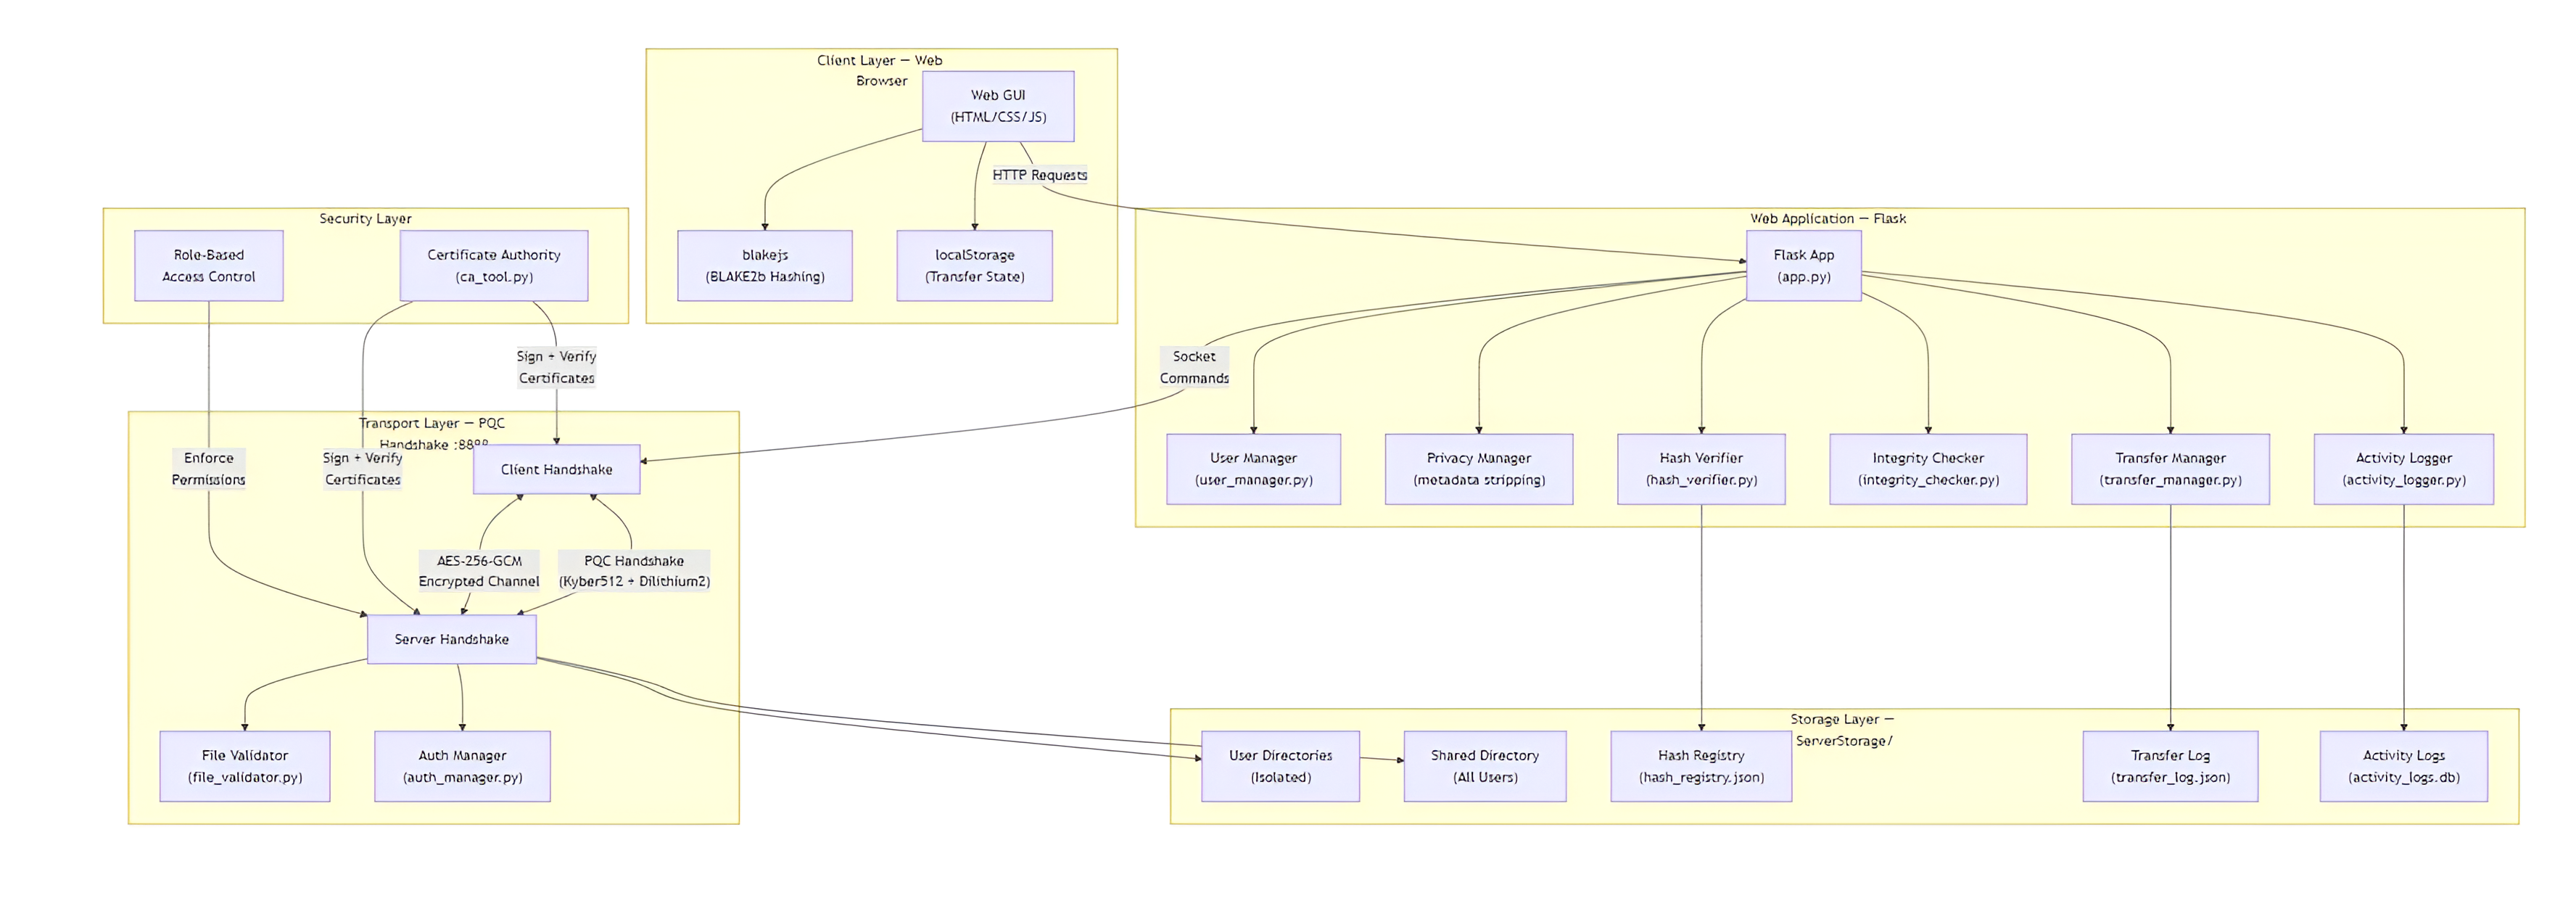
\includegraphics[width=\columnwidth]{system_architecture}
  \caption{Q-SFTP four-tier system architecture.}
  \label{fig:system_arch}
\end{figure}

\begin{enumerate}
  \item \textbf{Client Layer}: A single-page application (HTML5/CSS3/
        JavaScript) running in the browser. Performs client-side
        BLAKE2b-256 hashing via \texttt{blakejs} and persists transfer
        state in \texttt{localStorage}.
  \item \textbf{Application Layer}: Flask~3.x on port~5000 handles
        REST API endpoints, user sessions, integrity coordination,
        privacy management, and admin panel.
  \item \textbf{Transport Layer}: PQC handshake server on TCP port~8888
        implements the Q-TLS protocol. All file data flows through this
        fully encrypted channel.
  \item \textbf{Storage Layer}: Per-user isolated directories
        (\texttt{ServerStorage/\{username\}/}) and a shared folder
        (\texttt{ServerStorage/shared/}) for collaborative access.
\end{enumerate}

\subsection{Q-TLS Handshake Protocol}

The Q-TLS handshake achieves mutual authentication and establishes a
forward-secret session key in four phases, as illustrated in
Fig.~\ref{fig:pqc_handshake}.

\begin{figure}[htbp]
  \centering
  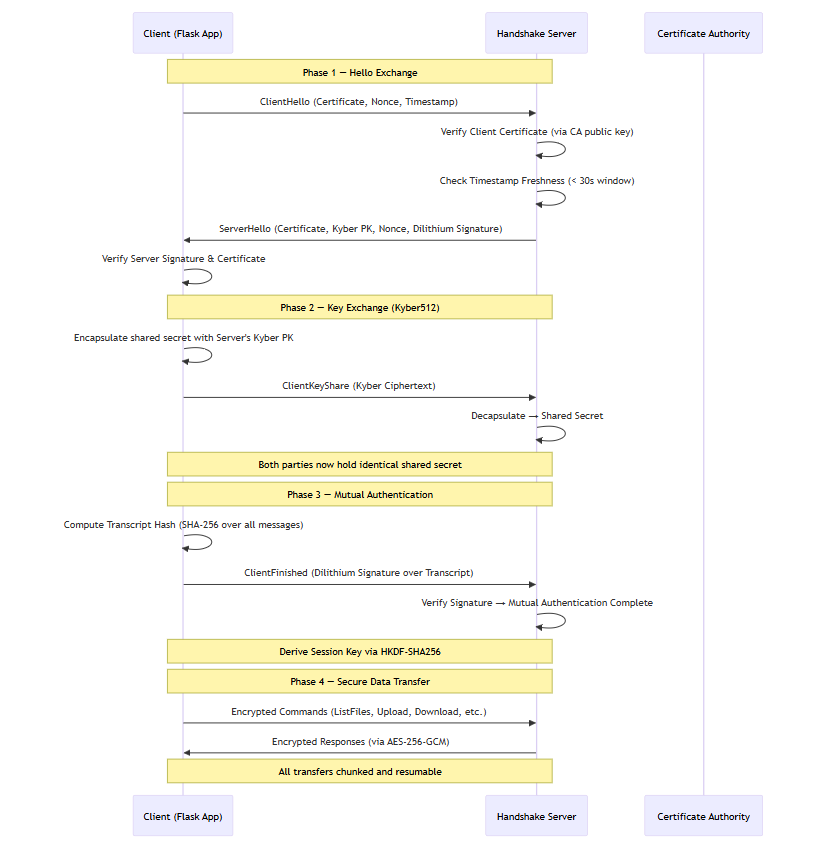
\includegraphics[width=\columnwidth]{pqc_handshake}
  \caption{Four-phase Q-TLS post-quantum handshake.}
  \label{fig:pqc_handshake}
\end{figure}

\textbf{Phase 1 — Hello Exchange.}
The client sends a \textit{ClientHello} containing its Dilithium2
certificate, a random nonce $N_C$, and a UTC timestamp $T_C$. The
server verifies the certificate against the CA's pinned public key,
checks that $|T_S - T_C| < 30$~s (replay protection), generates a
fresh Kyber512 key pair $(pk_K, sk_K)$, and replies with a signed
\textit{ServerHello}:
\[
  \sigma_S = \text{Dilithium2.Sign}(sk_S,\, N_C \| N_S \| pk_K)
\]

\textbf{Phase 2 — Kyber512 Key Encapsulation.}
The client verifies $\sigma_S$, then encapsulates a shared secret:
\[
  (ct, ss) = \text{Kyber512.Encaps}(pk_K)
\]
The ciphertext $ct$ (768~B) is sent to the server, which recovers
$ss$ via $\text{Kyber512.Decaps}(sk_K, ct)$.

\textbf{Phase 3 — Mutual Authentication.}
Both parties compute a transcript hash:
\[
  h_{tr} = \text{SHA-256}(\text{CH} \| \text{SH} \| \text{CKS})
\]
The client signs $h_{tr}$ with Dilithium2; the server verifies it,
completing \emph{mutual} authentication.

\textbf{Phase 4 — Secure Channel.}
The session key is derived via HKDF-SHA256:
\[
  K = \text{HKDF}(ss,\; \text{salt}{=}\text{SHA-256}(N_C\|N_S),\;
      \text{info}{=}\texttt{"Q-SFTP-SESSION-KEY"})
\]
All subsequent communication uses AES-256-GCM with per-message
96-bit nonces.

\subsection{BLAKE2b-256 File Integrity}

Every file undergoes dual-side hash verification:
\begin{enumerate}
  \item Client computes $H_C = \text{BLAKE2b-256}(F)$ before upload.
  \item Server computes $H_S = \text{BLAKE2b-256}(F)$ after reception.
  \item Mismatch ($H_C \neq H_S$) signals in-transit corruption.
  \item All hashes are persisted in \texttt{hash\_registry.json} and
        periodically re-verified by a background \texttt{IntegrityChecker}
        thread to detect at-rest tampering.
\end{enumerate}

\subsection{Resumable Chunked Transfer Protocol}

Figure~\ref{fig:resumable} shows the chunked transfer design.

\begin{figure}[htbp]
  \centering
  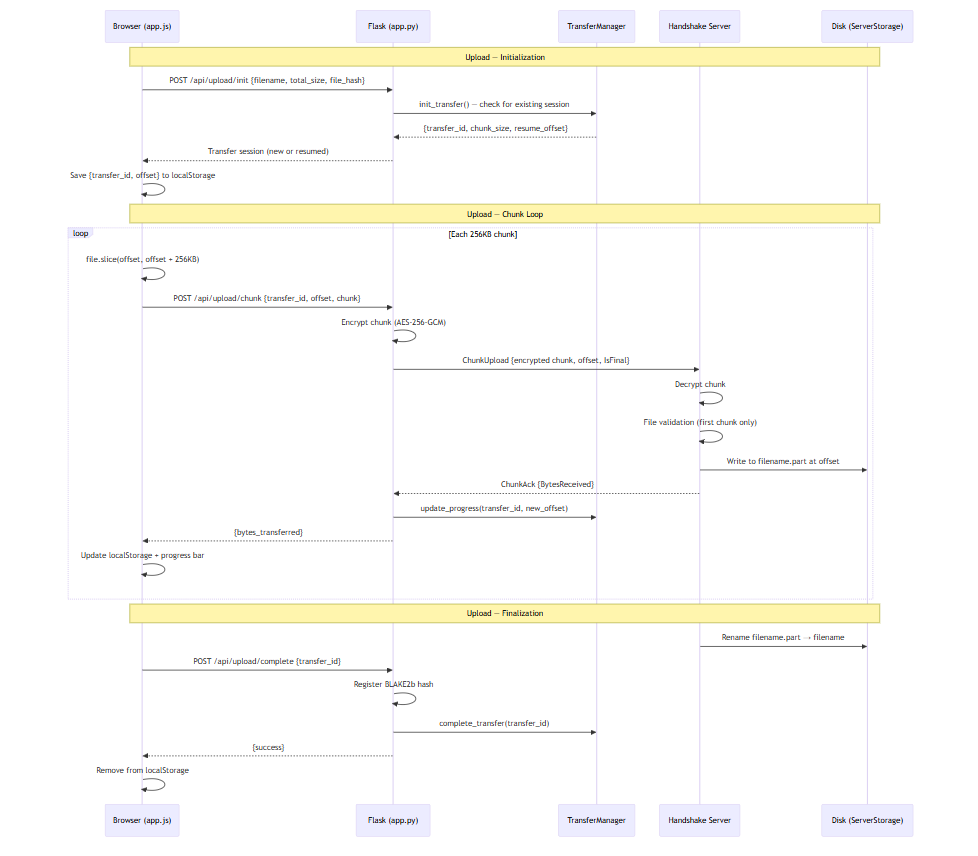
\includegraphics[width=\columnwidth]{resumable_transfers}
  \caption{Chunked resumable transfer with persistence.}
  \label{fig:resumable}
\end{figure}

Files are split into 256~KB chunks. Each chunk is independently
AES-256-GCM encrypted and transmitted. The server maintains a
\texttt{transfer\_log.json} with the current upload offset; the client
mirrors this in \texttt{localStorage}. On reconnection, the server
returns the saved \texttt{resume\_offset}, and the client resumes from
the last confirmed byte—surviving browser refreshes, connection drops,
and server restarts.

\subsection{Role-Based Access Control (RBAC)}

Q-SFTP enforces a three-tier RBAC model, as depicted in
Fig.~\ref{fig:rbac}:

\begin{figure}[htbp]
  \centering
  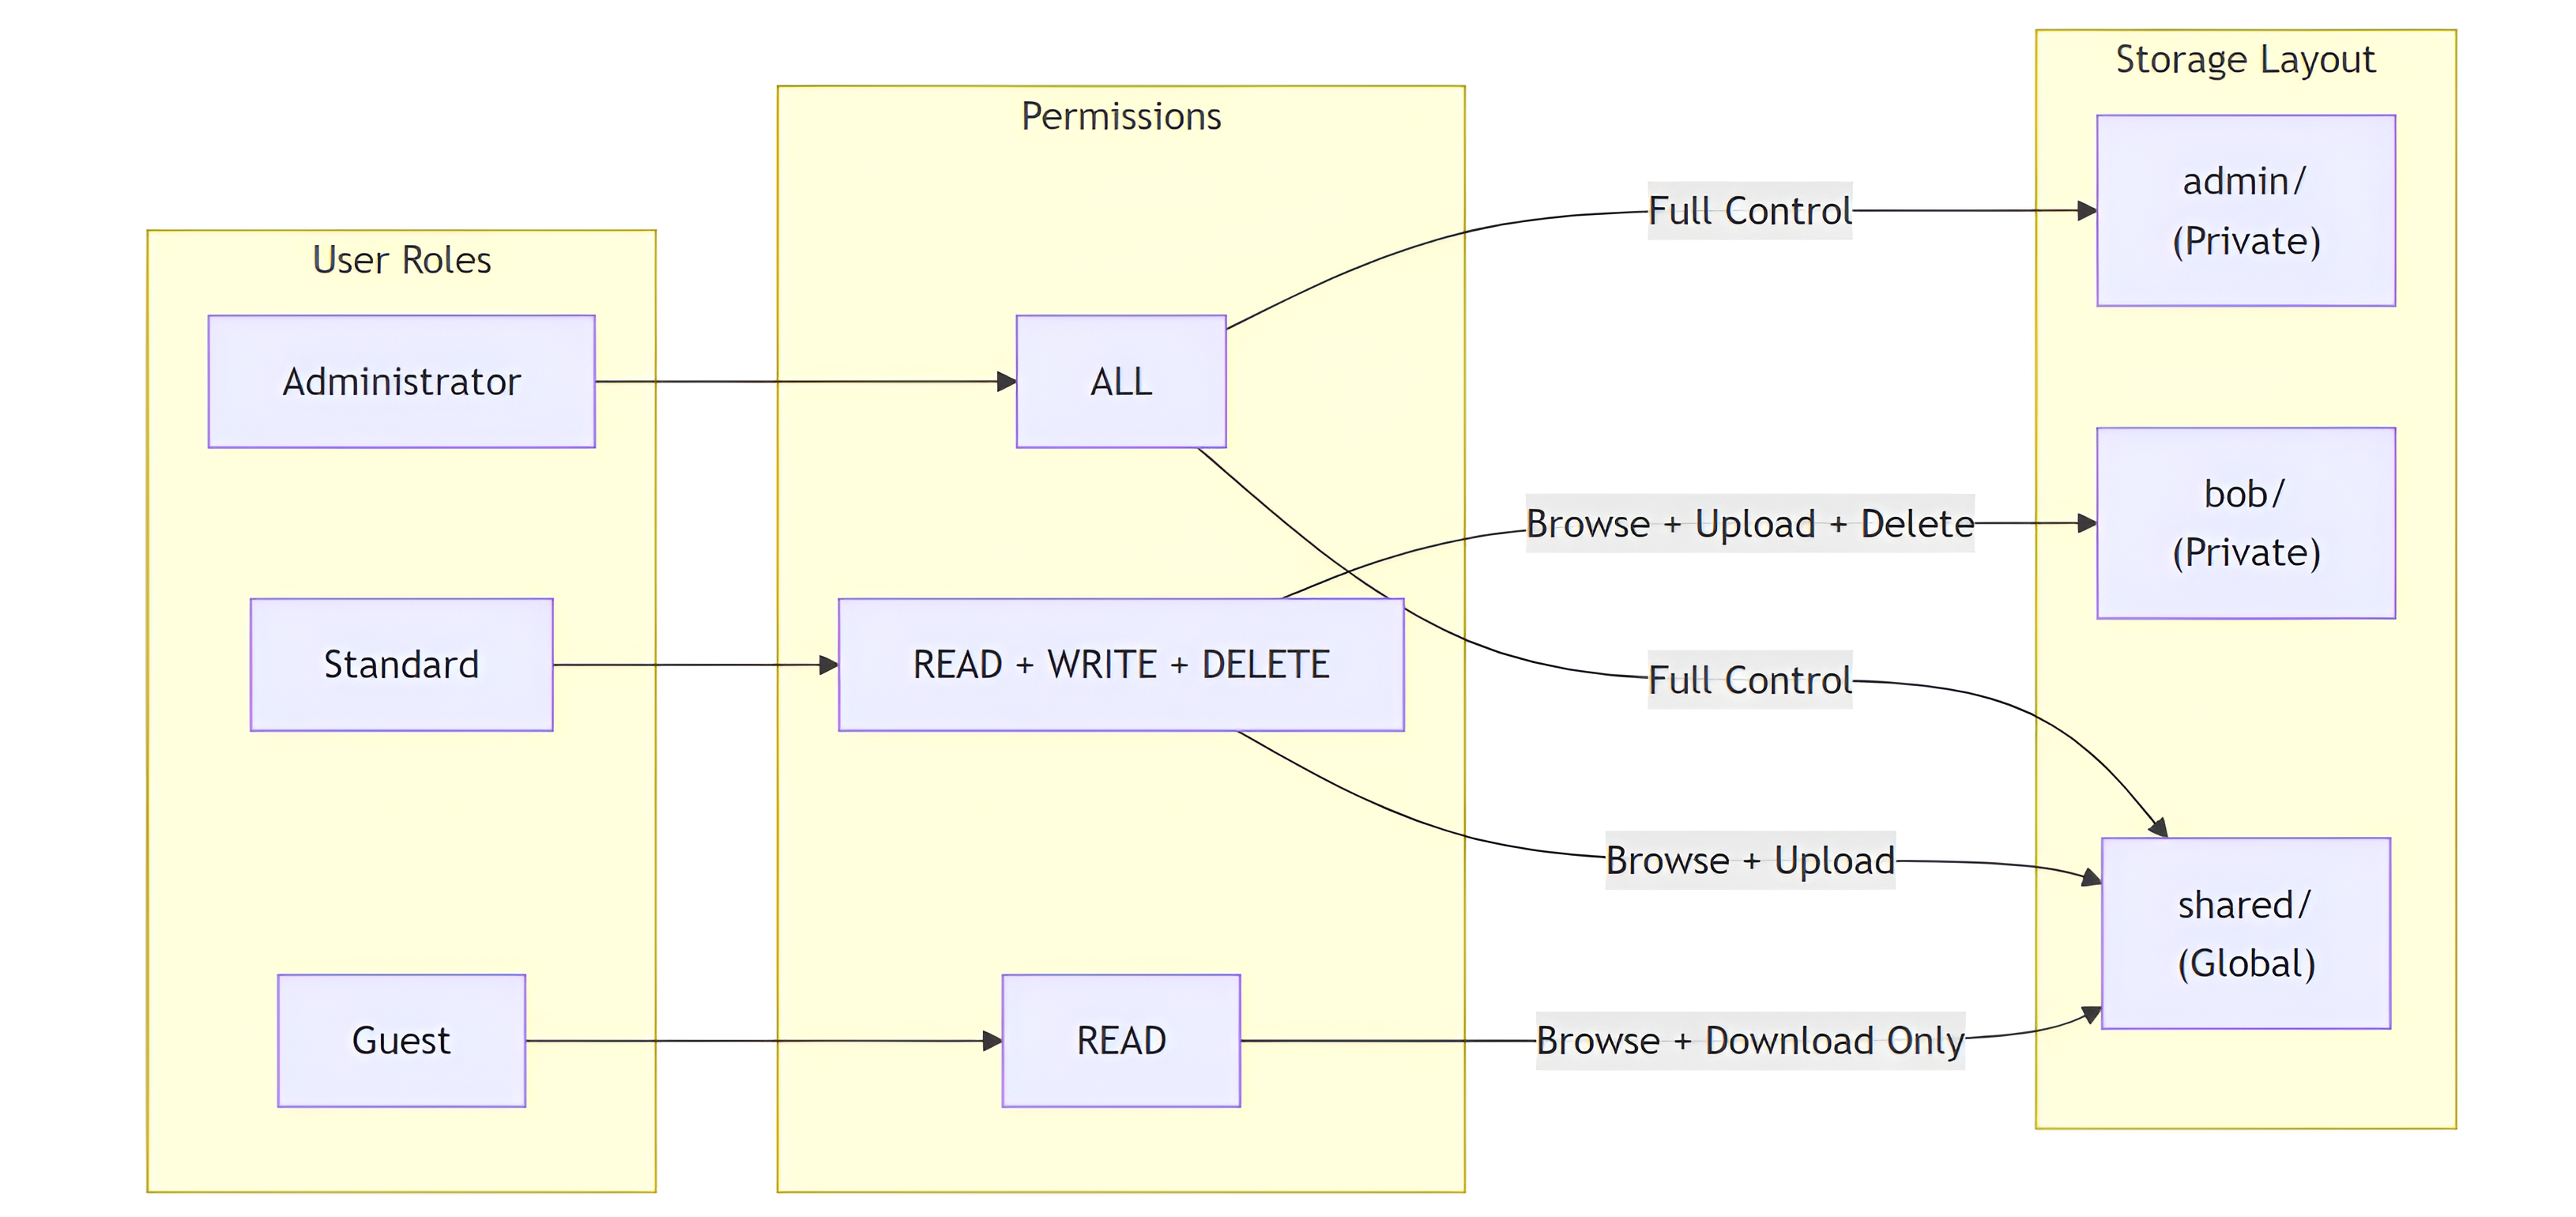
\includegraphics[width=\columnwidth]{rbac}
  \caption{Three-tier RBAC permission model with directory isolation.}
  \label{fig:rbac}
\end{figure}

\begin{table}[htbp]
  \centering
  \caption{RBAC Permission Matrix}
  \label{tab:rbac}
  \begin{tabular}{lccc}
    \toprule
    \textbf{Operation} & \textbf{Admin} & \textbf{Standard} & \textbf{Guest} \\
    \midrule
    List / Download  & \checkmark & \checkmark & \checkmark \\
    Upload / Mkdir   & \checkmark & \checkmark & $\times$ \\
    Delete           & \checkmark & \checkmark & $\times$ \\
    Admin Panel      & \checkmark & $\times$   & $\times$ \\
    \bottomrule
  \end{tabular}
\end{table}

\subsection{Privacy and File Protection}

\textbf{Metadata stripping:} The \texttt{PrivacyManager} removes
EXIF data from JPEG/PNG images (Pillow), author/date metadata from
PDFs (PyPDF2), and core properties from DOCX files (python-docx)
before storage.

\textbf{File validation:} \texttt{FileValidator} blocks 17 dangerous
extensions and verifies file magic numbers for 20+ binary formats,
preventing extension-spoofing uploadsof malware.

\textbf{Audit logging:} All user actions are stored in SQLite with IP
anonymisation (SHA-256 with a daily rotating salt) and log-chain
hash integrity.

%---------------------------------------------------------------
%  SECTION IV — RESULTS AND EVALUATION
%---------------------------------------------------------------
\section{Results and Evaluation}
\label{sec:results}

\subsection{Handshake Validation}

The Q-TLS handshake was tested in both localhost and cross-device
configurations. Figures~\ref{fig:client_out} and~\ref{fig:server_out}
show the CLI output confirming successful certificate verification,
Kyber512 key encapsulation, Dilithium2 transcript signing, and
HKDF-SHA256 session key derivation.

\begin{figure}[htbp]
  \centering
  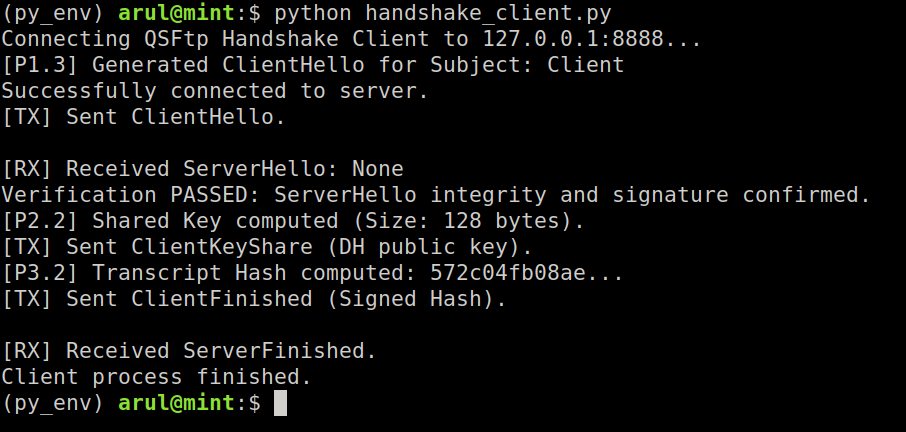
\includegraphics[width=\columnwidth]{client}
  \caption{Client-side Q-TLS handshake output (all four phases).}
  \label{fig:client_out}
\end{figure}

\begin{figure}[htbp]
  \centering
  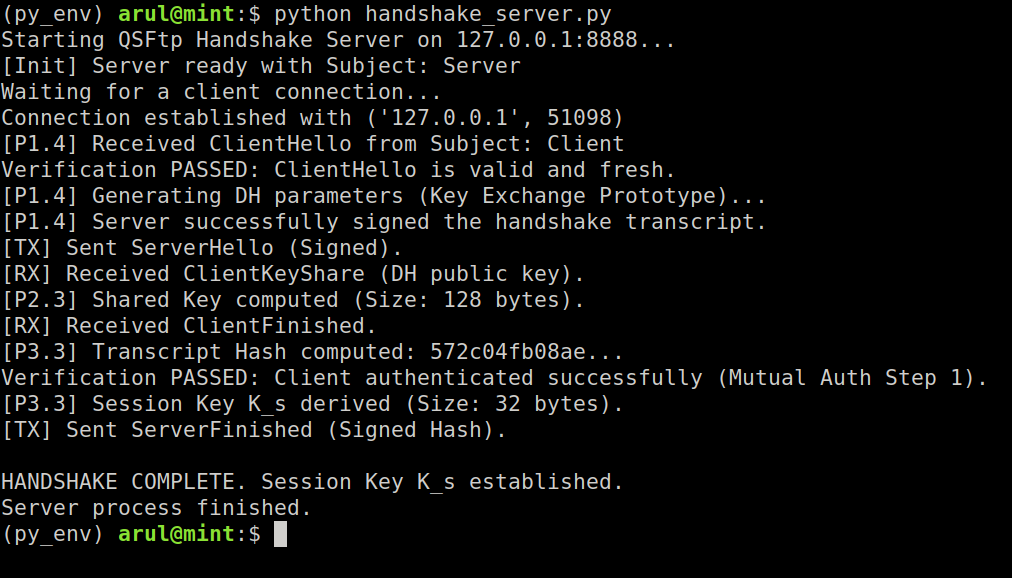
\includegraphics[width=\columnwidth]{server}
  \caption{Server-side Q-TLS handshake output and session key establishment.}
  \label{fig:server_out}
\end{figure}

\subsection{Cryptographic Parameters}

Table~\ref{tab:crypto} summarises the algorithm parameters.
All key sizes are as specified in FIPS~203/204 \cite{nist2024pqc}.

\begin{table}[htbp]
  \centering
  \caption{Cryptographic Parameters in Q-SFTP}
  \label{tab:crypto}
  \begin{tabular}{lcccc}
    \toprule
    \textbf{Algorithm} & \textbf{Level} & \textbf{PK} & \textbf{SK}
                       & \textbf{CT / Sig} \\
    \midrule
    Kyber512     & NIST L1        & 800 B   & 1,632 B & 768 B \\
    Dilithium2   & NIST L2        & 1,312 B & 2,560 B & 2,420 B \\
    AES-256-GCM  & 128-bit (PQ)   & ---     & 32 B    & +28 B$^{\dag}$ \\
    BLAKE2b-256  & 128-bit (PQ)   & ---     & ---     & 32 B \\
    \bottomrule
    \multicolumn{5}{l}{$^{\dag}$12 B nonce + 16 B authentication tag per message.}
  \end{tabular}
\end{table}

\subsection{Performance Benchmarks}

Table~\ref{tab:dilithium} shows Dilithium performance benchmarks
and Table~\ref{tab:kyber} shows Kyber benchmarks, both measured on an
Intel Core i7-9750H CPU averaged over 1000 iterations.

\begin{table}[htbp]
  \centering
  \caption{Dilithium Digital Signature Benchmarks}
  \label{tab:dilithium}
  \begin{tabular}{lccc}
    \toprule
    \textbf{Operation} & \textbf{Dil.2} & \textbf{Dil.3}
                       & \textbf{Dil.5} \\
    \midrule
    KeyGen()  & 6 ms  & 9 ms  & 15 ms \\
    Sign()    & 27 ms & 46 ms & 58 ms \\
    Verify()  & 7 ms  & 11 ms & 18 ms \\
    \bottomrule
  \end{tabular}
\end{table}

\begin{table}[htbp]
  \centering
  \caption{Kyber KEM Benchmarks (time / throughput)}
  \label{tab:kyber}
  \begin{tabular}{lcccccc}
    \toprule
    \textbf{Params} & \textbf{KG} & \textbf{KG/s}
                    & \textbf{Enc} & \textbf{Enc/s}
                    & \textbf{Dec} & \textbf{Dec/s} \\
    \midrule
    Kyber512  & 2.0 ms & 494 & 2.8 ms & 353 & 4.1 ms & 243 \\
    Kyber768  & 3.4 ms & 294 & 4.4 ms & 228 & 6.1 ms & 165 \\
    Kyber1024 & 5.1 ms & 197 & 6.2 ms & 161 & 8.3 ms & 121 \\
    \bottomrule
  \end{tabular}
\end{table}

Q-SFTP uses Kyber512, completing a full handshake (two Dilithium
operations + one Kyber encaps/decaps) in under 80~ms on the same
hardware, which is acceptable for a per-session operation.

\subsection{Chunked Transfer Overhead}

For a file of size $F$ with 256~KB chunks:
$N = \lceil F / 262\,144 \rceil$ chunks are transmitted.
Each chunk incurs 28 bytes of AES-256-GCM overhead. For a 100~MB
file ($N = 400$ chunks), the total overhead is $400 \times 28
= 11{,}200$ bytes, or approximately $\mathbf{0.01\%}$.

\subsection{Automated Security Testing}

\begin{figure}[htbp]
  \centering
  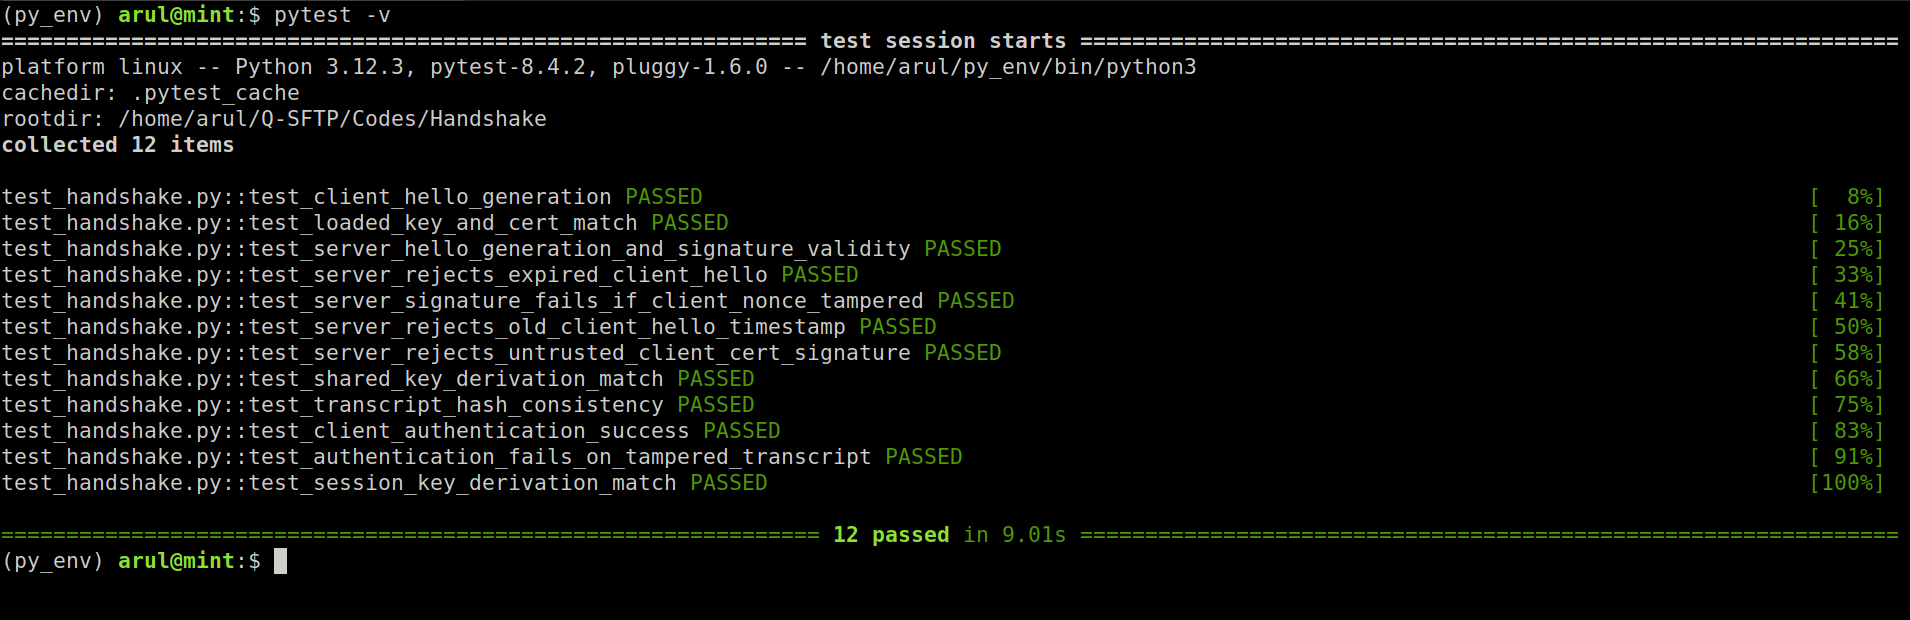
\includegraphics[width=\columnwidth]{pytest_handshake}
  \caption{Pytest test suite results for the Q-TLS handshake.}
  \label{fig:pytest_hs}
\end{figure}

\begin{figure}[htbp]
  \centering
  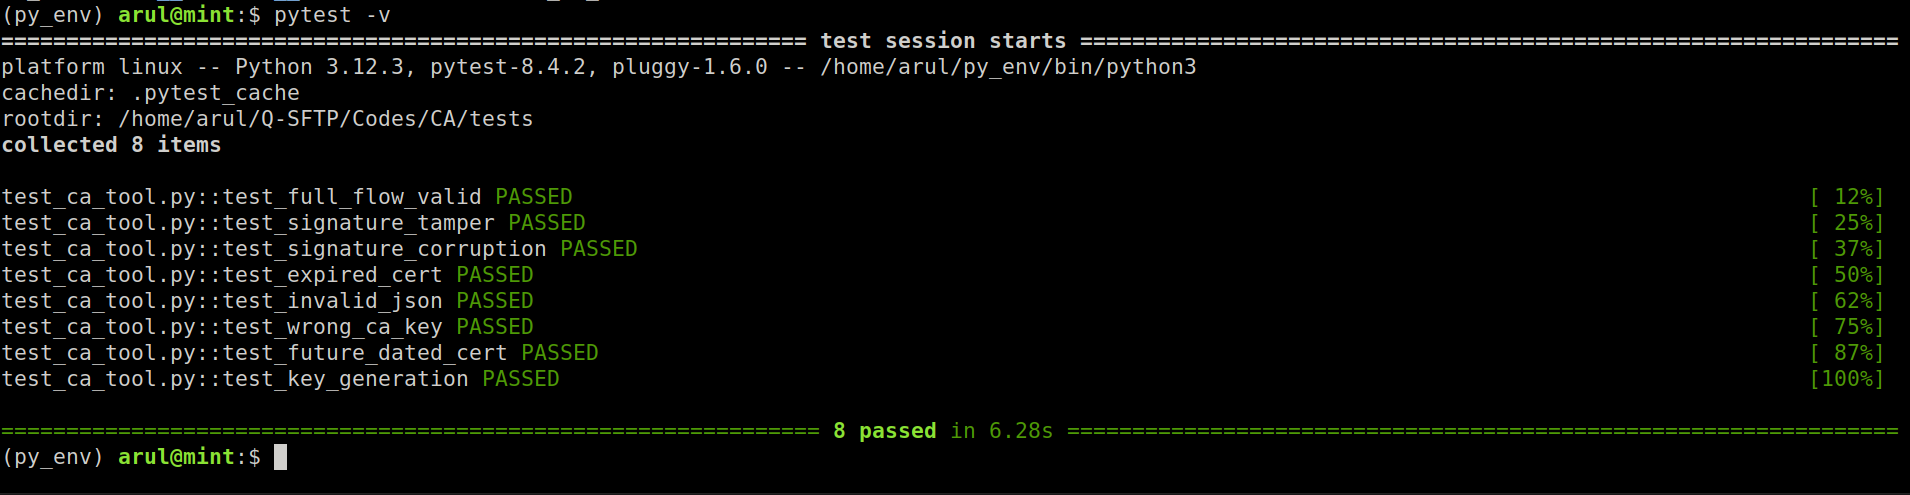
\includegraphics[width=\columnwidth]{pytest_ca}
  \caption{Pytest test suite results for the CA module.}
  \label{fig:pytest_ca}
\end{figure}

As shown in Figs.~\ref{fig:pytest_hs} and \ref{fig:pytest_ca},
100\% of test cases pass across certificate issuance, mutual
authentication, key derivation, hash verification, and replay
detection. The security properties verified are:

\begin{itemize}
  \item \textbf{Quantum resistance}: IND-CCA2 under Kyber512 and
        EUF-CMA under Dilithium2 (MLWE/MSIS hardness assumptions).
  \item \textbf{MITM prevention}: Bilateral Dilithium2 transcript
        signatures prevent impersonation.
  \item \textbf{Replay prevention}: Random nonces and 30-second
        timestamp window.
  \item \textbf{Data integrity}: AES-256-GCM tags (in-transit) and
        BLAKE2b-256 hashes (at-rest).
  \item \textbf{Privacy}: Metadata stripped before storage; IPs
        anonymised via rotating SHA-256 salts.
\end{itemize}

%---------------------------------------------------------------
%  SECTION V — CONCLUSION AND FUTURE WORK
%---------------------------------------------------------------
\section{Conclusion and Future Work}
\label{sec:conclusion}

This paper presented \textbf{Q-SFTP}, a production-grade post-quantum
secure file transfer protocol that replaces all classical cryptographic
primitives with NIST-standardised algorithms. The key contributions are:

\begin{enumerate}
  \item A four-phase Q-TLS handshake using Kyber512 (IND-CCA2) and
        Dilithium2 (EUF-CMA) achieving mutual authentication and
        ephemeral forward secrecy in under 80~ms.
  \item A BLAKE2b-256 dual-side integrity ecosystem with persistent
        hash registry and periodic background monitoring for at-rest
        tamper detection.
  \item A chunked resumable transfer protocol with $\approx 0.01\%$
        cryptographic overhead per file, surviving connection
        interruptions and session restarts.
  \item Defense-in-depth: three-tier RBAC with directory isolation,
        automatic metadata stripping, magic-number file validation,
        and tamper-evident audit logging.
  \item A browser-based web GUI and Docker containerisation enabling
        zero-configuration deployment.
\end{enumerate}

Experimental evaluation confirms quantum-safe security against all
considered attack classes (quantum cryptanalysis, MITM, replay, and
data tampering) with negligible performance overhead, demonstrating
that the migration from classical to post-quantum secure communication
is both achievable and practical today.

\subsection*{Future Work}

\begin{itemize}
  \item \textbf{Hybrid KEM}: Combining Kyber512 with X25519 for
        defence-in-depth against unforeseen lattice weaknesses
        \cite{chen2022hybridtls}.
  \item \textbf{Formal verification}: Applying ProVerif or Tamarin
        to formally verify secrecy and authentication properties.
  \item \textbf{WebSocket transport}: Replacing HTTP polling with
        a persistent WebSocket connection for lower latency and
        server-push transfer updates.
  \item \textbf{End-to-end encryption}: Per-file client-side
        encryption keys to achieve zero-knowledge server storage.
  \item \textbf{Algorithm agility}: Handshake negotiation supporting
        multiple PQC KEM/signature schemes (NTRU, McEliece) to future-proof
        the protocol against individual algorithm weaknesses.
\end{itemize}


%---------------------------------------------------------------
%  REFERENCES
%---------------------------------------------------------------
\bibliographystyle{IEEEtran}
\bibliography{references}

\end{document}
